% Created 2016-11-01 Tue 09:39
\documentclass[presentation,bigger]{beamer}
\usepackage[utf8]{inputenc}
\usepackage[T1]{fontenc}
\usepackage{fixltx2e}
\usepackage{graphicx}
\usepackage{grffile}
\usepackage{longtable}
\usepackage{wrapfig}
\usepackage{rotating}
\usepackage[normalem]{ulem}
\usepackage{amsmath}
\usepackage{textcomp}
\usepackage{amssymb}
\usepackage{capt-of}
\usepackage{hyperref}
\mode<beamer>{\usetheme{Madrid}}
\usetheme{default}
\author{Martin Zimmer Kristensen}
\date{\today}
\title{Dynamic Conditional Random Fields}
\subtitle{Factorized Probabilistic Models for Labeling and Segmenting Sequence Data}
\hypersetup{
 pdfauthor={Martin Zimmer Kristensen},
 pdftitle={Dynamic Conditional Random Fields},
 pdfkeywords={},
 pdfsubject={},
 pdfcreator={Emacs 24.5.2 (Org mode 8.3.6)}, 
 pdflang={English}}
\begin{document}

\maketitle
\begin{frame}{Outline}
\setcounter{tocdepth}{1}
\tableofcontents
\end{frame}

\section{Introduction}
\label{sec:orgheadline9}
\begin{frame}[label={sec:orgheadline1}]{Sequential Data}
\begin{block}{Part-of-speech Tagging}
The \alert{[DT]} little \alert{[JJ]} dog \alert{[NN]} was \alert{[VBD]} furious \alert{[JJ]} and \alert{[CC]} barked \alert{[VBD]} at \alert{[IN]} the \alert{[DT]} large \alert{[JJ]} human \alert{[NN]}
\end{block}
\begin{block}{Noun-phrase Chunking}
The \alert{[B-NP]} little \alert{[I-NP]} dog \alert{[I-NP]} was \alert{[O]} furious \alert{[O]} and \alert{[O]} barked \alert{[O]} at \alert{[O]} the \alert{[B-NP]} large \alert{[I-NP]} human \alert{[I-NP]}
\end{block}
\end{frame}
\begin{frame}[label={sec:orgheadline2}]{Sequential Data}
\begin{block}{Other}
\begin{itemize}
\item Named Entity Recognition
\item Speech Recognition
\end{itemize}
\end{block}
\end{frame}
\begin{frame}[label={sec:orgheadline3}]{Motivation}
\begin{block}{Generative Models (HMMs, DBNs):}
\begin{itemize}
\item The joint probability \(p(x,y)\)
\begin{itemize}
\item Generate features
\item Unnecessary when only segmenting and labeling data
\item Assumptions among features to achieve tractability
\begin{itemize}
\item Hurts performance
\end{itemize}
\end{itemize}
\end{itemize}
\end{block}
\end{frame}
\begin{frame}[label={sec:orgheadline4}]{Motivation}
\begin{block}{Discriminative Models (CRFs, DCRFs):}
\begin{itemize}
\item The conditional probability: \(p(y|x)\)
\begin{itemize}
\item Dependencies among \(x\) not explicitly modeled
\item No assumptions among (interdependent) features
\begin{itemize}
\item Capitalization, prefixes, suffixes, neighboring words\ldots{}
\end{itemize}
\item Unseen words can be labeled by using interdependent features
\end{itemize}
\end{itemize}
\end{block}
\end{frame}

\begin{frame}[label={sec:orgheadline5}]{Conditional Random Fields}
\begin{definition}[Conditional Random Fields]
\begin{itemize}
\item Let \(G\) be an undirected model over sets of random variables \(y\) and \(x\)
\item Let \(C = \{\{y_c, x_c\}\}\) be the set of cliques in \(G\)
\item Conditional probability defined as:
\end{itemize}
\[ p_\Lambda(y|x) = \dfrac{1}{Z(x)}\prod_{c \in C} \Phi (y_c, x_c) \]
\begin{itemize}
\item \(\Phi\) is a potential function
\item \(Z(x)\) is the partition function
\end{itemize}
\end{definition}
\end{frame}
\begin{frame}[label={sec:orgheadline6}]{Conditional Random Fields}
\begin{block}{Feature Functions}
\begin{itemize}
\item Potentials factorize according to a set of weights \(\{\lambda_k\}\) and feature functions \(\{f_k\}\):
\end{itemize}
\[ \Phi(y_c,x_c) = exp\Bigg(\sum_k \lambda_kf_k(y_c,x_c)\Bigg) \]
\end{block}
\end{frame}
\begin{frame}[label={sec:orgheadline7}]{Linear-chain CRF}
\begin{figure}[htb]
\centering
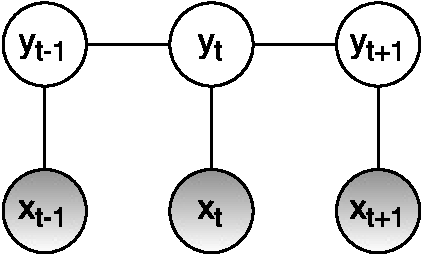
\includegraphics[width=5cm]{figures/LCRF.pdf}
\end{figure}
\begin{itemize}
\item Previous applications use linear-chain CRF
\begin{itemize}
\item Tractable exact inference algorithms
\end{itemize}
\item Conditional version of hidden Markov models
\item Feature functions can be described as:
\[ f_k(y_{t-1},y_t,x,t) \]
\end{itemize}
\end{frame}
\begin{frame}[label={sec:orgheadline8}]{Linear-chain CRF}
\begin{block}{Feature Functions:}
\begin{itemize}
\item \(f(y_{t-1}, y_t, x, t) = 1\):
\begin{itemize}
\item \emph{iff} \(y_{t-1} = adjective\), \(y_t = \textit{proper noun}\), and \(x_t\) begins with a capital letter.
\end{itemize}
\item \(f(y_{t-1}, y_t, x, t) = 1\):
\begin{itemize}
\item \emph{iff} \(y_t = \textit{organization}\), \(x_{t} = \textit{``New''}\), \(x_{t+1} = \textit{``York''}\), and \(x_{t+2} = \textit{``Times''}\)
\end{itemize}
\end{itemize}
\end{block}
\end{frame}
\section{Dynamic Conditional Random Fields}
\label{sec:orgheadline20}
\begin{frame}[label={sec:orgheadline10}]{Key Contributions}
\begin{itemize}
\item Dynamic Conditional Random Fields (DCRF)
\begin{itemize}
\item Generalization of linear-chain CRFs
\item Similar to DBNs
\item Factorial CRF
\item Inference approximation algorithm for complex models
\end{itemize}
\end{itemize}
\begin{figure}[htb]
\centering
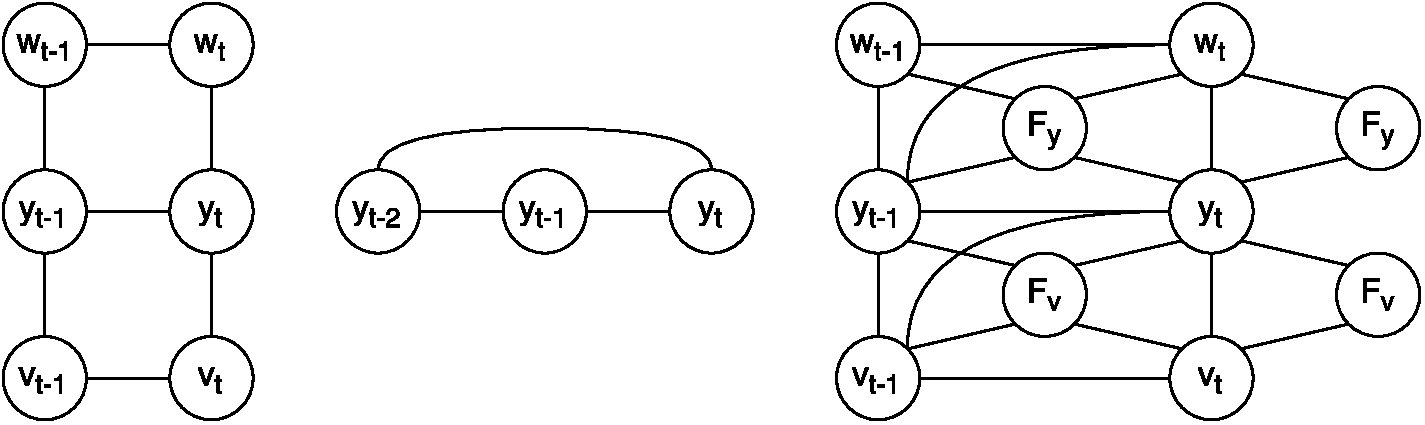
\includegraphics[width=\textwidth]{figures/DCRF.pdf}
\end{figure}
\end{frame}

\begin{frame}[label={sec:orgheadline11}]{Dynamic Conditional Random Fields}
\begin{itemize}
\item \(y_{ij}\) is the variable \(j\) at time \(i\)
\end{itemize}
\begin{definition}[Clique Index]
\begin{itemize}
\item Given a time \(t\), denote any variable \(y_{ij}\) in \(y\) by:
\begin{itemize}
\item Its index \(j\) in \(y_i\)
\item Its time offset \(\Delta t = i-t\)
\end{itemize}
\item \(c = \{(\Delta t, j)\}\) is a clique index
\item \(y_{t,c}\) is the set of variables in clique index \(c\) at time \(t\)
\end{itemize}
\end{definition}
\end{frame}
\begin{frame}[label={sec:orgheadline12}]{Dynamic Conditional Random Fields}
\begin{definition}[Dynamic Conditional Random Field]
\begin{itemize}
\item \(p(y|x) = \dfrac{1}{Z(x)}\displaystyle \prod_{t}\prod_{c \in C} \text{exp}\Bigg(\sum_k \lambda_k f_k(y_{t,c},x,t)\Bigg)\)
\item where \(Z(x)\) is the partition function
\end{itemize}
\end{definition}
\end{frame}
\begin{frame}[label={sec:orgheadline13}]{Factorial Conditional Random Field}
\begin{itemize}
\item A DCRF which has linear chains of labels with edges between cotemporal labels.
\end{itemize}
\begin{figure}[htb]
\centering
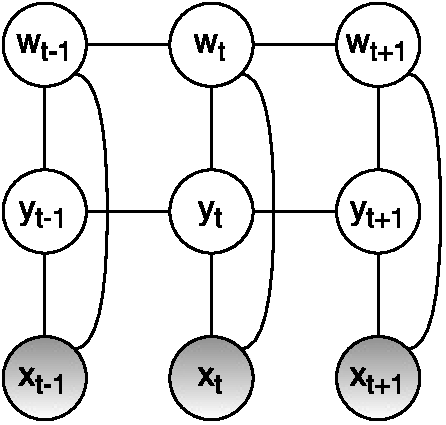
\includegraphics[width=5cm]{figures/FCRF.pdf}
\end{figure}
\end{frame}
\begin{frame}[label={sec:orgheadline14}]{Factorial Conditional Random Field}
\begin{block}{Cliques}
\begin{itemize}
\item The cliques are of the form:
\begin{itemize}
\item Within-chain edges: \text{ }\text{ }\(\{(0,\ell),(1,\ell)\}\)
\item Between-chain edges: \(\{(0,\ell),(0,\ell+1)\}\)
\end{itemize}
\end{itemize}
\end{block}
\end{frame}
\begin{frame}[label={sec:orgheadline15}]{Factorial Conditional Random Field}
\begin{definition}[Factorial CRF]
\(p(x|y) = \dfrac{1}{Z(x)}\Bigg(\displaystyle\prod_{t=1}^{T-1}\prod_{\ell=1}^{L}\Phi_\ell(y_{\ell,t},y_{\ell,t+1},x,t)\Bigg)\Bigg(\prod_{t=1}^{T}\prod_{\ell=1}^{L-1}\Psi_\ell(y_{\ell,t},y_{\ell+1,t},x,t)\Bigg)\)
\begin{itemize}
\item \(\{\Phi_\ell\}\) are the factors over within-chain edges
\item \(\{\Psi_\ell\}\) are the factors over between-chain edges
\item \(Z(x)\) is the partition function.
\end{itemize}
\end{definition}
\end{frame}
\begin{frame}[label={sec:orgheadline16}]{Factorial Conditional Random Field}
\begin{block}{Factors}
\begin{itemize}
\item The factors are modeled using features \(\{f_k\}\) and weights \(\{\lambda_k\}\) of \(G\) as:
\[\Phi_\ell(y_{\ell,t},y_{\ell,t+1},x,t) = \text{exp}\Bigg\{\sum_k\lambda_k f_k(y_{\ell,t},y_{\ell,t+1},x,t)\Bigg\}\text{,}\]
\[\Psi_\ell(y_{\ell,t},y_{\ell+1,t},x,t) = \text{exp}\Bigg\{\sum_k\lambda_k f_k(y_{\ell,t},y_{\ell+1,t},x,t)\Bigg\}\text{.}\]
\end{itemize}
\end{block}
\end{frame}
\begin{frame}[label={sec:orgheadline17}]{Inference}
\begin{itemize}
\item Exact inference intractable for some models
\item Approximate inference using loopy belief propagation
\end{itemize}
\end{frame}
\begin{frame}[label={sec:orgheadline18}]{Inference}
\begin{block}{Loopy Belief Propagation}
\begin{itemize}
\item Message from node \(x_u\) to node \(x_v\):
\[ m_{x_u}(x_v) \]
\item Value of \(m_{x_u}(x_v)\):
\begin{itemize}
\item The belief of \(x_u\) about the probability \(p(x_v)\)
\end{itemize}
\item Iteratively send messages until convergence or early cutoff
\item Different schedules can be applied
\begin{itemize}
\item Random
\item Tree-based (send messages from leaves to root and back)
\end{itemize}
\end{itemize}
\end{block}
\end{frame}
\begin{frame}[label={sec:orgheadline19}]{Parameter Estimation}
\begin{itemize}
\item Given training data \(D = \{x^{(i)},y^{(i)}\}^N_{i=1}\)
\begin{itemize}
\item Find s set of parameters \(\Lambda = \{\lambda_k\}\)
\end{itemize}
\item Use L-BFGS
\end{itemize}
\end{frame}
\section{Experiments}
\label{sec:orgheadline26}
\begin{frame}[label={sec:orgheadline21}]{Experiments}
\begin{block}{Noun-phrase Chunking}
The \alert{[B-NP]} little \alert{[I-NP]} dog \alert{[I-NP]} was \alert{[O]} furious \alert{[O]} and \alert{[O]} barked \alert{[O]} at \alert{[O]} the \alert{[B-NP]} large \alert{[I-NP]} human \alert{[I-NP]}
\end{block}
\begin{block}{Usual approach:}
\begin{enumerate}
\item POS tagging
\item Noun-phrase Chunking
\end{enumerate}
\end{block}
\begin{block}{Challenge:}
\begin{itemize}
\item Mistakes in POS tagging will cascade onto noun-phrase chunking
\end{itemize}
\end{block}
\end{frame}
\begin{frame}[label={sec:orgheadline22}]{Experiments}
\begin{block}{Data:}
\begin{itemize}
\item CoNLL 2000
\end{itemize}
\end{block}
\begin{block}{Approach:}
\begin{itemize}
\item Use a factorial CRF to jointly do POS and chunking
\end{itemize}
\end{block}
\begin{block}{Compare to:}
\begin{itemize}
\item CRF+CRF
\item Brill+CRF
\begin{itemize}
\item Brill tagger trained on over four times more data including the CoNLL 2000
\item More than 40.000 sentences
\end{itemize}
\end{itemize}
\end{block}
\end{frame}
\begin{frame}[label={sec:orgheadline23}]{Results}
\begin{figure}[htb]
\centering
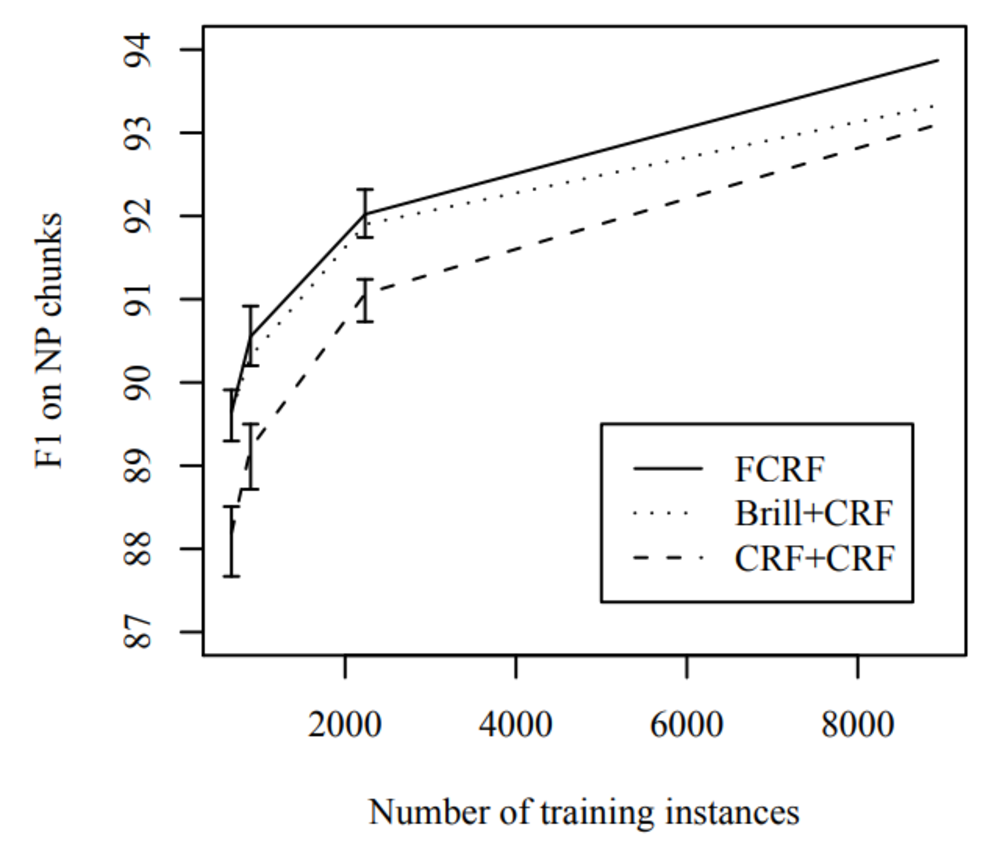
\includegraphics[width=8cm]{figures/npgraph.pdf}
\end{figure}
\end{frame}
\begin{frame}[label={sec:orgheadline24}]{Results}
\begin{figure}[htb]
\centering
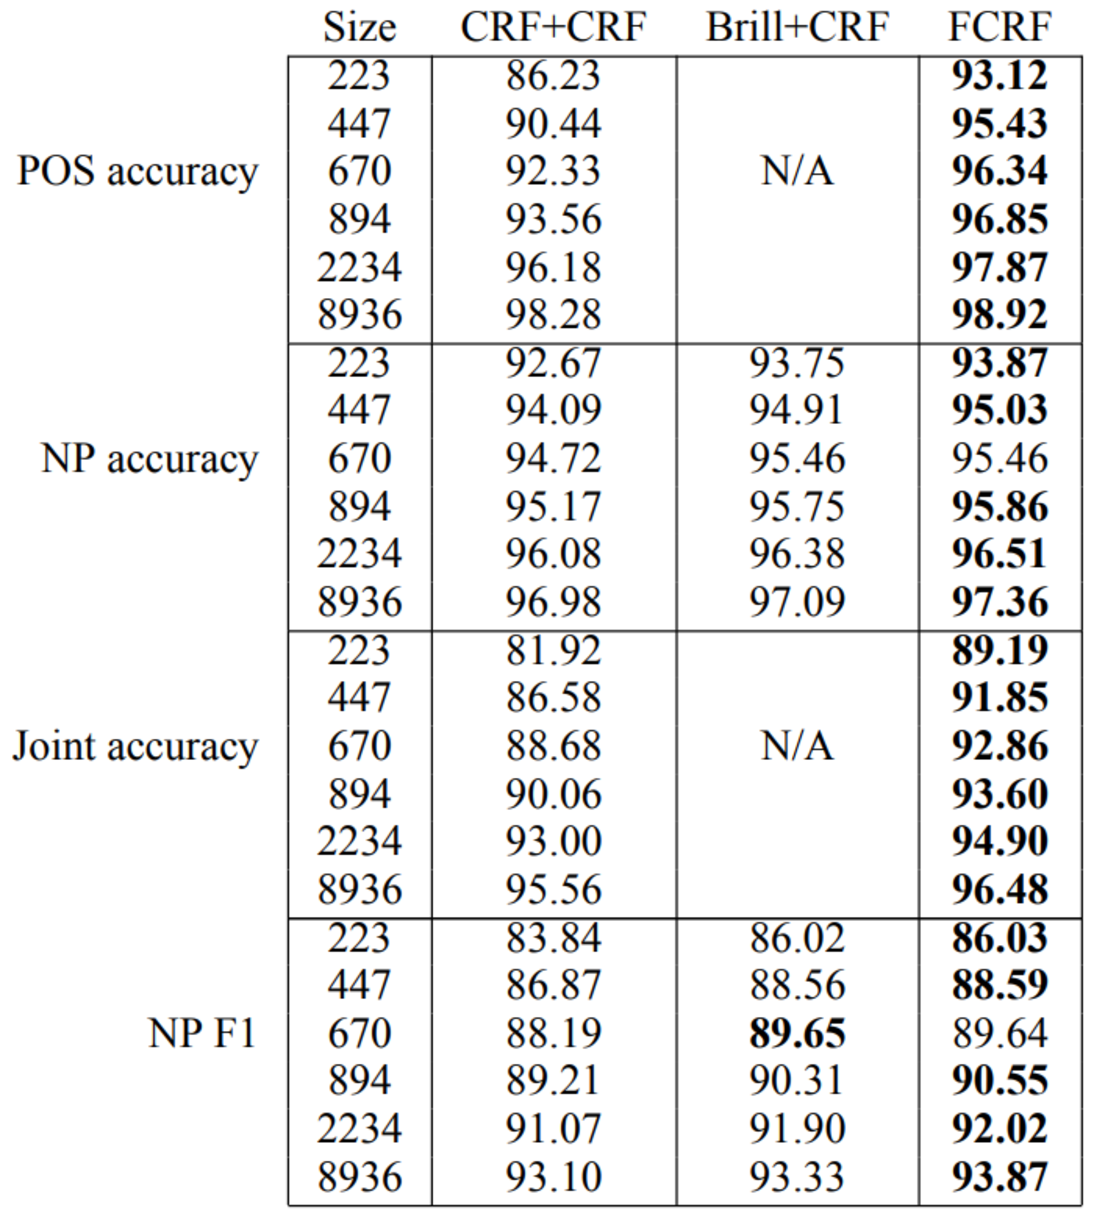
\includegraphics[width=7cm]{figures/nptab.pdf}
\end{figure}
\end{frame}
\begin{frame}[label={sec:orgheadline25}]{Inference Algorithms}
\begin{figure}[htb]
\centering
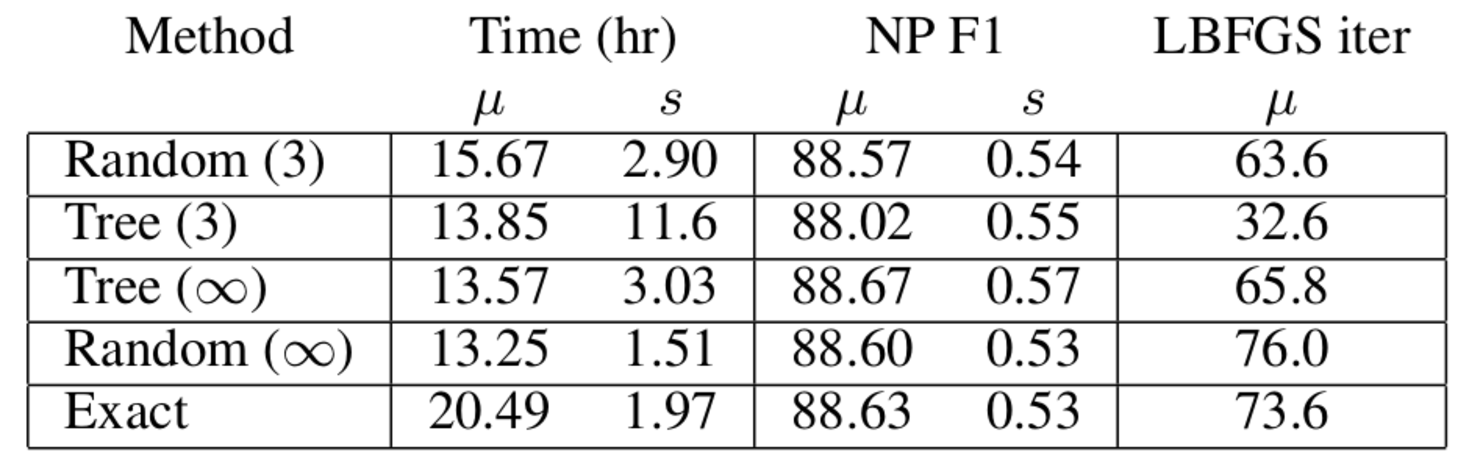
\includegraphics[width=\textwidth]{figures/npinf.pdf}
\end{figure}
\end{frame}
\section{Conclusions}
\label{sec:orgheadline28}
\begin{frame}[label={sec:orgheadline27}]{Conclusions}
\begin{itemize}
\item Jointly perform several labeling tasks at once perform better than the sequential approach
\begin{itemize}
\item Useful for many NLP tasks
\end{itemize}
\item Loopy belief propagation:
\begin{itemize}
\item Reduces training time
\item Performs equally to exact inference
\end{itemize}
\end{itemize}
\end{frame}
\end{document}